\documentclass[14pt]{extarticle} 
\usepackage{amsmath,mathtools,amsfonts,amsthm,amssymb,hyperref}
\usepackage{wasysym,geometry,bussproofs,latexsym,parskip,bookmark}
\usepackage{mathtools,float}
\newtheorem{defn}{Definition}
\newtheorem{thm}{Theorem}
\newtheorem{claim}{Claim}
\newtheorem{lemma}{Lemma}
\hypersetup{colorlinks,allcolors=blue,linktoc=all}
\geometry{a4paper} 
\geometry{margin=0.5in}
\title{Math for CS 2015/2019 solutions to ``In-Class Problems Week 8, Mon. (Session 18)''}
\author{https://github.com/spamegg1}
\begin{document}
\maketitle
\tableofcontents

\section{Problem 1}
For each of the binary relations below, state whether it is a strict partial order, a weak partial order, an equivalence relation, or none of these. If it is a partial order, state whether it is a linear order. If it is none, indicate which of the axioms for partial-order and equivalence relations it violates.

Weak partial order: reflexive, antisymmetric, transitive.

Strict partial order: irreflexive, asymmetric, transitive.

Equivalence relation: reflexive, symmetric, transitive.

Linear order: partial order (weak or strict) with trichotomy.

\subsection{(a)}
The superset relation $\supseteq$ on the power set $pow\{1, 2, 3, 4, 5\}$.
\begin{proof}
It is reflexive: $a \supseteq a$ is true for all $a \in pow\{1, 2, 3, 4, 5\}$.

It is transitive: for all $a, b, c \in pow\{1, 2, 3, 4, 5\}$, if $a \supseteq b$ and $b \supseteq c$ then $a \supseteq c$ is true.

It is antisymmetric: for all $a, b \in pow\{1,2,3,4,5\}$, if $a \neq b$ and $a \supseteq b$, then $a \supset b$ and therefore $b \nsupseteq a$.

This is a WEAK PARTIAL ORDER!
\end{proof}

\subsection{(b)}
The relation between any two nonnegative integers $a$ and $b$ such that $a \equiv b \mod 8$.
\begin{proof}
It is reflexive: for all nonnegative integers $a$, $a \equiv a \mod 8$ is true.

It is symmetric: for all nonnegative integers $a$ and $b$, if $a \equiv b \mod 8$, then 8 divides $(a - b)$, so 8 also divides $(b-a)$, therefore $b \equiv a \mod 8$.

It is transitive: for all nonnegative integers $a, b$ and $c$, if $a \equiv b \mod 8$ and $b \equiv c \mod 8$, then 8 divides both $(a-b)$ and $(b-c)$, so 8 also divides their sum $(a - b) + (b - c) = (a - c)$, therefore $a \equiv c \mod 8$.

This is an EQUIVALENCE RELATION!
\end{proof}

\subsection{(c)}
The relation between propositional formulas $G$ and $H$ such that [$G$ IMPLIES $H$] is valid.
\begin{proof}
It is reflexive: for all propositional formulas $G$, $G$ IMPLIES $G$ is valid.

Below, let $P, Q$ be propositional variables, and let TRUE denote the formula $P$ IFF $P$, and let FALSE denote the formula $P$ IFF NOT$(P)$. So TRUE is true under every assignment, and FALSE is false under every assignment.

It is not symmetric: FALSE IMPLIES TRUE is valid, but TRUE IMPLIES FALSE is not valid.

It is not asymmetric because it's reflexive.

It is not antisymmetric: ($P$ IFF $P$) IMPLIES ($Q$ IFF $Q$) is valid, but ($Q$ IFF $Q$) IMPLIES ($P$ IFF $P$) is also valid!

It is transitive: for all propositional formulas $F, G, H$, if $F$ IMPLIES $G$ is valid, and $G$ IMPLIES $H$ is valid, then $F$ IMPLIES $H$ is also valid.

This is NOT A PARTIAL ORDER!
\end{proof}

\subsection{(d)}
The relation between propositional formulas $G$ and $H$ such that [$G$ IFF $H$] is valid.
\begin{proof}
It is reflexive: for all propositional formulas $G$, $G$ IFF $G$ is valid.

It is symmetric: for all propositional formulas $G, H$, if $G$ IFF $H$ is valid, then $H$ IFF $G$ is also valid.

It is transitive: for all propositional formulas $F, G, H$, if $F$ IFF $G$ is valid, and $G$ IFF $H$ is valid, then $F$ IFF $H$ is also valid.

This is an EQUIVALENCE RELATION!
\end{proof}

\subsection{(e)}
The relation ‘beats’ on Rock, Paper, and Scissors (for those who don’t know the game Rock, Paper, Scissors, Rock beats Scissors, Scissors beats Paper, and Paper beats Rock).
\begin{proof}
It is irreflexive: for all $x \in \{R, P, S\}$ $x$ does not beat $x$.

It is antisymmetric: for all $x, y \in \{R, P, S\}$ if $x$ beats $y$, then $y$ does not beat $x$.

It is not transitive: Rock beats Scissors, and Scissors beats Paper, but Rock does not beat Paper.

This is NOT A PARTIAL ORDER!
\end{proof}

\subsection{(f)}
The empty relation on the set of real numbers.
\begin{proof}
It's irreflexive, asymmetric, transitive. 

This is a STRICT PARTIAL ORDER!
\end{proof}

\subsection{(g)}
The identity relation on the set of integers.
\begin{proof}
It is reflexive: for all integers $x$, $x=x$ is true.

It is symmetric: for all integers $x, y$, if $x = y$ then $y = x$.

It is transitive: for all integers $x, y, z$, if $x = y$ and $y = z$ then $x = z$.

This is an EQUIVALENCE RELATION!
\end{proof}

\subsection{(h)}
The divisibility relation on the integers, $\mathbb{Z}$.
\begin{proof}
It is reflexive: for all $x \in \mathbb{Z}$, $x$ divides $x$. (Yes this is true even when $x = 0$.)

It is not symmetric: 3 divides 6, but 6 does not divide 3.

It is not asymmetric because it's reflexive.

It is not antisymmetric: $2$ divides $-2$, and $-2$ divides $2$.

This is NOT A PARTIAL ORDER!
\end{proof}

\section{Problem 2}
The proper subset relation, $\subset$, defines a strict partial order on the subsets of $[1..6]$, that is, on $pow([1..6])$.

\subsection{(a)}
What is the size of a maximal chain in this partial order? Describe one.
\begin{proof}
It is 7: 
$$
\emptyset \subset \{1\} \subset \{1, 2\} \subset \{1, 2, 3\} \subset \{1, 2, 3, 4\} \subset \{1, 2, 3, 4, 5\} \subset \{1, 2, 3, 4, 5, 6\}
$$
\end{proof}

\subsection{(b)}
Describe the largest antichain you can find in this partial order.
\begin{proof}
Subsets of $[1..6]$ that have the same size form antichains. There are:

1 subset of $[1..6]$ with 0 elements,

6 subsets of $[1..6]$ with 1 elements,

15 subsets of $[1..6]$ with 2 elements,

21 subsets of $[1..6]$ with 3 elements,

15 subsets of $[1..6]$ with 4 elements,

6 subsets of $[1..6]$ with 5 elements,

1 subset of $[1..6]$ with 6 elements.

So the largest antichain is formed by the 21 3-element subsets of $[1..6]$.
\end{proof}

\subsection{(c)}
What are the maximal and minimal elements? Are they maximum and minimum?
\begin{proof}
The maximal and maximum element is $\{1,2,3,4,5,6\}$; the minimal and minimum element is $\emptyset$.
\end{proof}

\subsection{(d)}
Answer the previous part for the partial order on the set $pow([1..6]) - \emptyset$.
\begin{proof}
Now the maximal/maximum element is still $\{1,2,3,4,5,6\}$; however there is no minimum element. Instead there are 6 minimal elements: $\{1\}, \{2\}, \{3\}, \{4\}, \{5\}, \{6\}$.
\end{proof}

\section{Problem 3}
Let $S$ be a sequence of $n$ different numbers. A subsequence of $S$ is a sequence that can be obtained by deleting elements of $S$.

For example, if
$$
S = (6, 4, 7, 9, 1, 2, 5, 3, 8)
$$

Then 647 and 7253 are both subsequences of S (for readability, we have dropped the parentheses and commas in sequences, so 647 abbreviates (6, 4, 7), for example).

An increasing subsequence of $S$ is a subsequence of whose successive elements get larger. For example, 1238 is an increasing subsequence of $S$. Decreasing subsequences are defined similarly; 641 is a decreasing subsequence of $S$.

\subsection{(a)}
List all the maximum-length increasing subsequences of $S$, and all the maximum-length decreasing subsequences.
\begin{proof}
Maximum length increasing subsequences: 1258 1238

Maximum length decreasing subsequences: 641 642 643 653 753 953
\end{proof}

Now let $A$ be the set of numbers in $S$. (So $A$ is the integers $[1..9]$ for the example above.) There are two straightforward linear orders for $A$. The first is numerical order where $A$ is ordered by the $<$ relation. The second is to order the elements by which comes first in $S$; call this order $<_S$. So for the example above, we would have 
$$
6 <_S 4 <_S 7 <_S 9 <_S 1 <_S 2 <_S 5 <_S 3 <_S 8
$$
Let $\prec$ be the product relation of the linear orders $<_s$ and $<$. That is, is defined by the rule
$$
a \prec a' \Coloneqq a < a' \text{ AND } a <_S a'
$$
So $\prec$ is a partial order on $A$ (Section 9.9 in the course textbook).

\subsection{(b)}
Draw a diagram of the partial order, $\prec$, on $A$. What are the maximal and minimal elements?
\begin{proof}
8 and 9 are maximal elements. 1, 4, 6 are the minimal elements.
\begin{figure}[ht!]
\centering
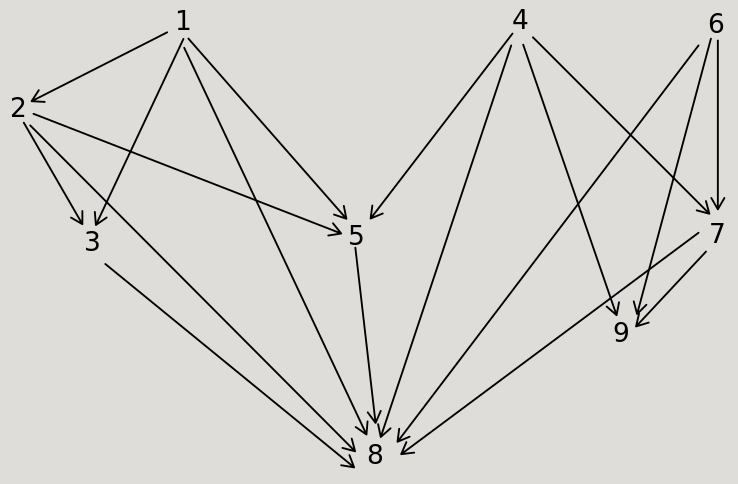
\includegraphics[scale=0.5]{partial-order.png}
\end{figure}
\end{proof}

\subsection{(c)}
Explain the connection between increasing and decreasing subsequences of $S$, and chains and antichains under $\prec$.
\begin{proof}
An increasing subsequence of $S$ is a chain of $\prec$.

A decreasing subsequence of $S$ is an antichain of $\prec$.
\end{proof}

\subsection{(d)}
Prove that every sequence, $S$, of length $n$ has an increasing subsequence of length greater than $\sqrt{n}$ or a decreasing subsequence of length at least $\sqrt{n}$.
\begin{proof}
Immediately follows from Dilworth's Lemma and part (c).
\end{proof}

\section{Problem 4}
For any total function $f: A \to B$ define a relation $\equiv_f$ by the rule:
$$
a \equiv_f a' \text{ iff } f(a) = f(a')
$$

\subsection{(a)}
Observe (and sketch a proof) that $\equiv_f$ is an equivalence relation on $A$.
\begin{proof}
1. For all $a \in A$, we have $f(a) = f(a)$, therefore $a \equiv_f a$. So $\equiv_f$ is reflexive.

2. Assume $a, b \in A$ and $a \equiv_f b$. Then by definition $f(a) = f(b)$. Then $f(b) = f(a)$. Therefore $b \equiv_f a$. So $\equiv_f$ is symmetric.

3. Assume $a,b,c \in A$ and $a \equiv_f b$ and $b \equiv_f c$. Then $f(a) = f(b)$ and $f(b) = f(c)$. Therefore $f(a) = f(c)$. So $a \equiv_f c$. So $\equiv_f$ is transitive.

4. By (1), (2), (3) $\equiv_f$ is an equivalence relation.
\end{proof}

\subsection{(b)}
Prove that every equivalence relation, $R$, on a set, $A$, is equal to $\equiv_f$ for the function $f: A \to pow(A)$ defined as
$$
f(a) \Coloneqq \{a' \in A \,\,|\,\, a R a'\}
$$
That is, $f(a) = R(a)$.
\begin{proof}
1. Assume $R$ is an equivalence relation on $A$. We want to show $R$ is equal to $\equiv_f$ for the function $f$ defined in the problem.

2. Assume $a, b \in A$. We want to show $a R b$ IFF $a \equiv_f b$.

3. Assume $a R b$. We want to show $f(a) = f(b)$.

4. To show $f(a) = f(b)$, we will show $f(a) \subseteq f(b)$ and $f(b) \subseteq f(a)$.

5. To show $f(a) \subseteq f(b)$, assume $x \in f(a)$. We want to show $x \in f(b)$.

6. By definition $f(a) = \{a' \in A \,\,|\,\, a R a'\}$. So $a R x$.

7. Since $R$ is symmetric, $x R a$.

8. Since $a R b$ and $R$ is transitive, $x R b$.

9. Again by symmetry, $b R x$.

10. By definition $f(b) = \{a' \in A \,\,|\,\, b R a'\}$. So $x \in f(b)$. This proves $f(a) \subseteq f(b)$.

11. The proof of $f(b) \subseteq f(a)$ is very similar. Therefore we have shown $f(a) = f(b)$.

12. Therefore we have shown that $a R b$ IMPLIES $a \equiv_f b$.

13. The proof of the converse $a \equiv_f b$ IMPLIES $a R b$ is very similar.

14. So we have shown $a R b$ IFF $a \equiv_f b$. Therefore $R$ is equal to $\equiv_f$.
\end{proof}

\end{document}
